\documentclass[../main.tex]{subfiles}

Este primer capítulo recoge lo esencial del trabajo. En él, se explica el contexto en el cual se enmarca el estudio, el problema a solucionar, la motivación del mismo y los objetivos extraídos del problema. Además, se presenta también cual será la estructura seguida en la memoria.

\section{Robótica Aérea} \label{section:intro-contexto}
El término \emph{robot} aparece por primera vez en 1920, en la obra teatral \emph{Rosum's Universal Robots} del escritor checo Karel Capek en cuyo idioma la palabra ``robota'' significa fuerza o servidumbre \cite{martin2007historia}. El nacimiento de la robótica y los robots surge asociado a la idea de trabajo y producción tras la Segunda Revolución Industrial y a lo largo del siglo XX. La automatización industrial de aquella época da lugar a los primeros sistemas de control automático que se extienden rápidamente a todos los sectores industriales, y que dan lugar a la robótica industrial tal como la conocemos hoy en día \cite{baturone2005robotica}. \\
El término \emph{robótica} es acuñado por Isaac Asimov, definiendo a la ciencia que estudia a los robots. El propio Asimov postuló también las Tres Leyes de la Robótica en su libro \emph{Yo Robot} publicado en 1950 \cite{martin2007historia}. El término ha evolucionado mucho desde sus inicios, hoy entendemos la robótica como la rama de la tecnología que estudia el diseño y construcción de máquinas capaces de desempeñar tareas realizadas por el ser humano o que requieren el uso de inteligencia \cite{rae}. Como se puede entender, la visión actual es mucho más amplia que en sus inicios y abarca muchas áreas de la ingeniería. \\
Existen diversas clasificaciones en función de su arquitectura, de su aplicación, de su cronología, etc. Una de estas clasificaciones distingue robots en función de su morfología \cite{de2006robotica}, que suele distinguir los siguientes tipos:

\begin{itemize}
    \item \textbf{Poliarticulados:} Son artilugios mecánicos y electrónicos destinados a realizar de forma automática determinados procesos de fabricación o manipulación. Suelen ser fijos, aunque también pueden realizar desplazamientos limitados y poseen un espacio de trabajo concreto y limitado. Los mejores ejemplos son los robots industriales, manipuladores o cartesianos.
    \item \textbf{Móviles:} Están provistos de algún tipo de mecanismo que les permite desplazarse autónomamente, como patas o ruedas, y reciben información de su entorno a través de sus propios sensores. Son ampliamente utilizados en el transporte de mercancías o en la exploración de lugares de difícil acceso. Pueden ser terrestres, acuáticos, aéreos o espaciales.
    \item \textbf{Androides:} Intentan reproducir total o parcialmente la forma y el comportamiento del ser humano. No solo imitan la apariencia humana (antropomorfismo), si no que emulan también la conducta de forma autónoma.
    \item \textbf{Zoomórficos:} Son aquellos que trata de reproducir en mayor o menor grado de realismo los sistemas de locomoción de diversos seres vivos. Este tipo podría incluir también a la morfología androide, en función del autor de la clasificación. Una subclasificación distingue entre robots caminadores y no caminadores.
\end{itemize}

Este trabajo se enmarca dentro de la robótica móvil, y más en concreto, dentro de la robótica aérea. La robótica aérea es la rama de la robótica que se encarga del estudio del comportamiento autónomo de aeronaves no tripuladas. Se entiende como una aeronave no tripulada (UAV, \emph{Unmanned Aerial Vehicle}, o más recientemente UAVS, \emph{Unmanned Aircraft Vehicle System}) a aquella que es capaz de realizar una misión sin necesidad de tener una tripulación embarcada \cite{barrientos2007vehiculos}. Otro término que también se utiliza con frecuencia es VANT, Vehículo Aéreo No Tripulado. \\

\begin{figure}[!ht]
    \centering
    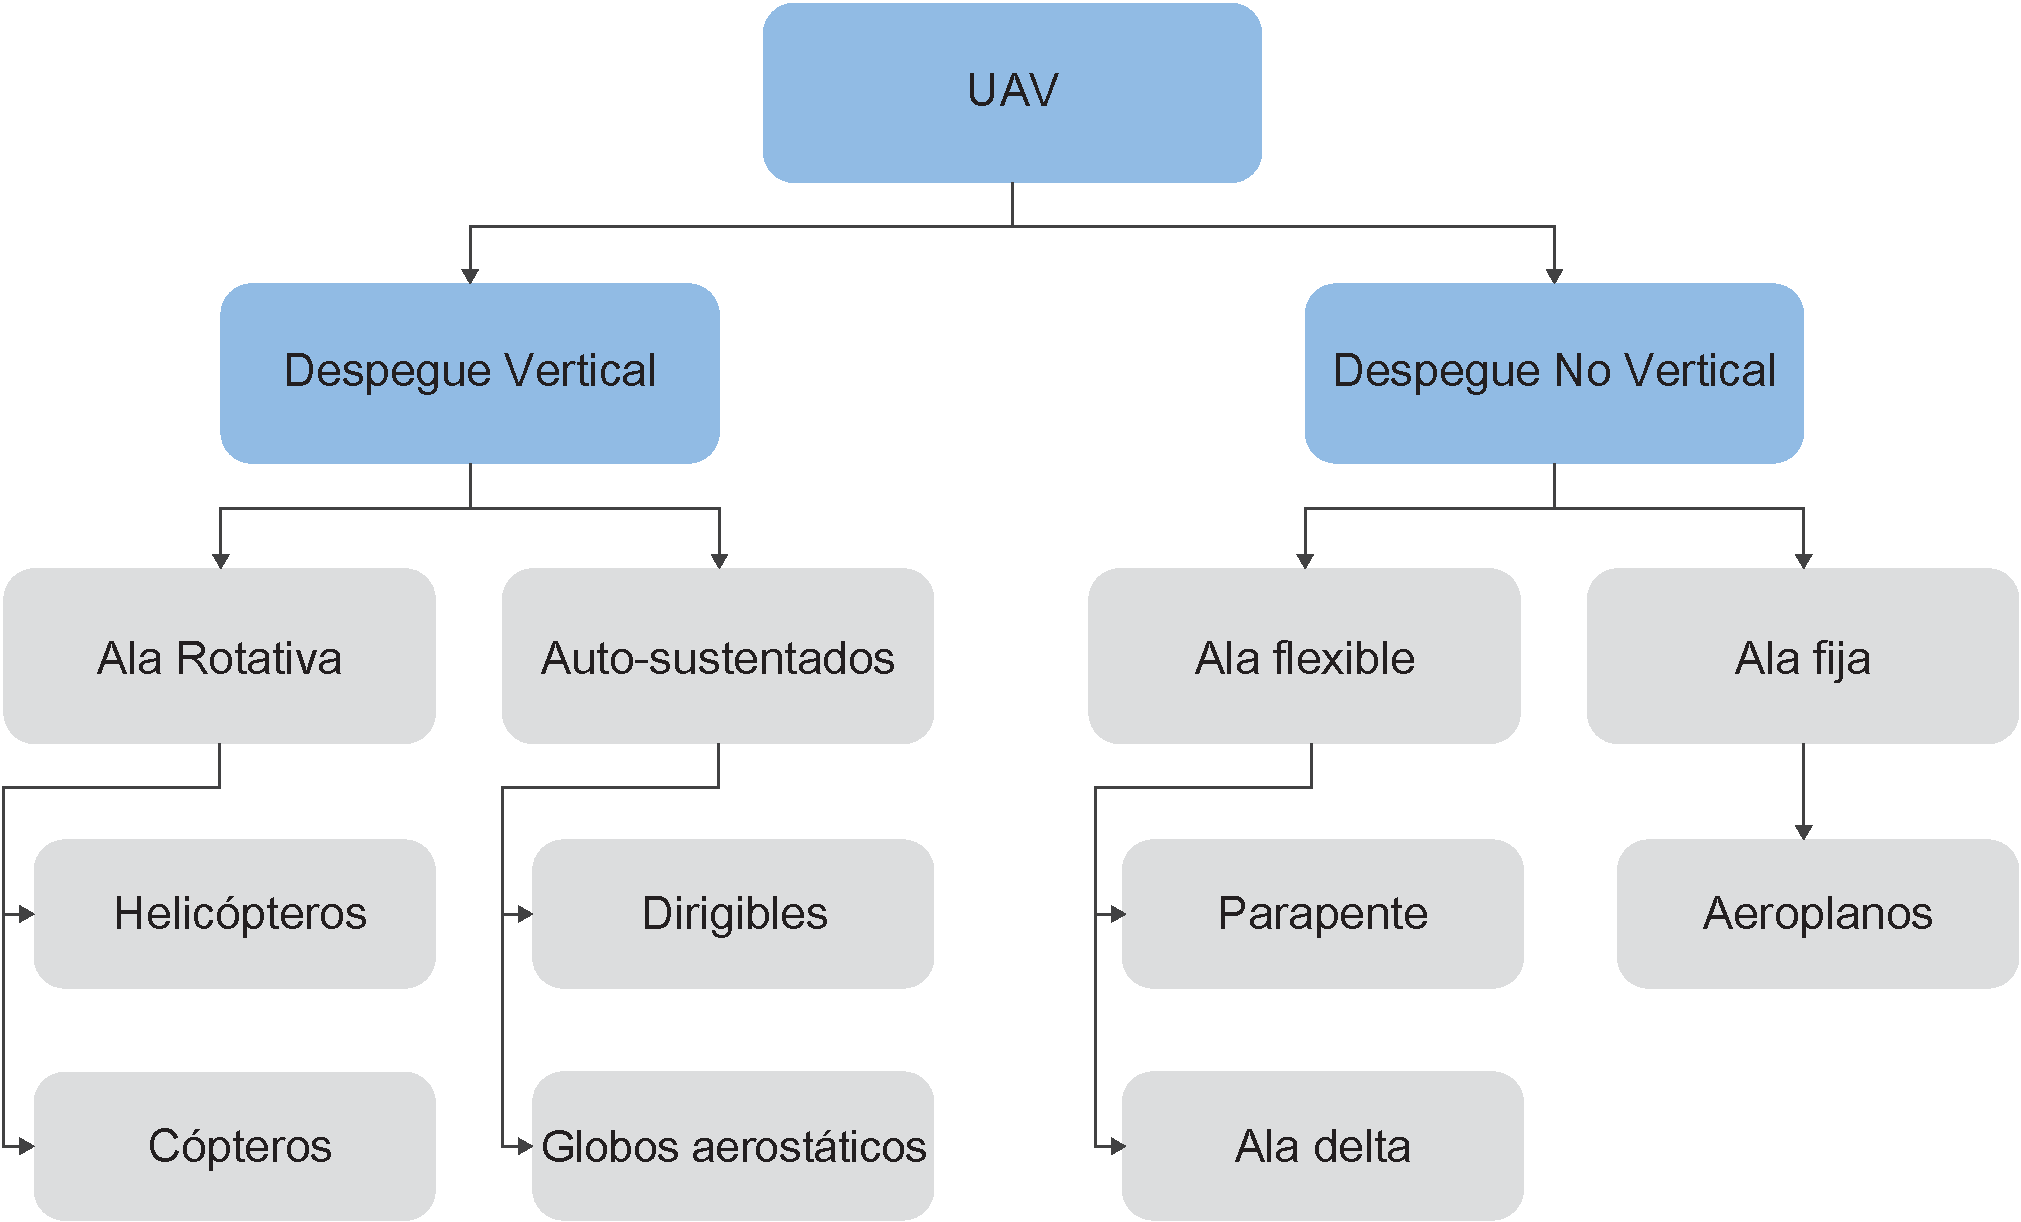
\includegraphics[width=\textwidth]{fig_tipos_auv.pdf}
    \caption{Clasificación de los UAV \cite{barrientos2007vehiculos}.}
    \label{fig:clasif-uav}
\end{figure}

A la hora de establecer una clasificación de los UAV es posible atender a diferentes criterios. Siguiendo la clasificación propuesta por \emph{Barrientos et al.} \cite{barrientos2007vehiculos} se distinguen aeronaves en función del tipo de despegue, que puede ser vertical o no. A su vez, podemos subdividir las aeronaves en función del origen de su sustentación o del tipo de ala que poseen. Esta clasificación se representa en la Figura \ref{fig:clasif-uav}, mientras que en la Figura \ref{fig:tipos-uav} se muestran ejemplos de los diferentes tipos de UAV.

\begin{figure}[ht]
    \begin{subfigure}{0.5\textwidth}
        \includegraphics[height=6cm, width=0.9\linewidth]{alafija.jpeg}
        \caption{Aeroplano.}
        \label{fig:tipo1}
    \end{subfigure}
    \begin{subfigure}{0.5\textwidth}
        \includegraphics[height=6cm, width=0.9\linewidth]{coptero.jpeg}
        \caption{Multicóptero.}
        \label{fig:tipo2}
    \end{subfigure}
     
    \caption{Tipos de UAV.}
    \label{fig:tipos-uav}
\end{figure}

\pagebreak

Otros criterios de clasificación pueden responder a las capacidades de vuelo como el alcance, la altitud, la autonomía o la carga máxima. A su vez, también se clasificar las aeronaves en función de la actividad que realizan. \\
Las principales aplicaciones se recogen en la siguiente lista:

\begin{itemize}
    \item Militar: de apoyo, de combate, de reconocimiento, etc.
    \item Transporte, tanto de mercancías o de personas.
    \item Seguridad, vigilancia y salvamento.
    \item Ocio y entretenimiento: en cine, en deporte, etc.
    \item Educación e investigación.
    \item Agropecuario: fumigación, control de recursos, etc.
    \item Cartografía, topografía y fotografía aérea.
\end{itemize}

La Figura \ref{fig:aplic-uav} recoge alguna de las principales aplicaciones mencionadas. \\


En la actualidad tiende a utilizarse el concepto de UAVS frente al de UAV. La extensión del concepto de vehículo a sistema refleja que el vehículo aéreo autónomo precisa para su funcionamiento de todo un sistema y no solo de la aeronave instrumentada. En concreto la instrumentación embarcada o segmento aire, debe verse complementada con la estación base o segmento tierra, debiéndose considerar las funcionalidades y características de ambos segmentos. Típicamente, el segmento tierra se compone de un ordenador donde se ejecuta un software tipo estación de tierra, mientras que el segmento aire se compone por una aeronave. La comunicación entre ellos se realiza a través de un protocolo de comunicaciones.

\begin{figure}[!ht]
    \begin{subfigure}{0.5\textwidth}
        \includegraphics[height=6cm, width=0.9\linewidth]{transporte.jpg}
        \caption{Transporte de mercancías \cite{tfg-diego}.}
        \label{fig:aplic1}
    \end{subfigure}
    \begin{subfigure}{0.5\textwidth}
        \includegraphics[height=6cm, width=0.9\linewidth]{entretenimiento.jpg}
        \caption{Spot publicitario \cite{tfg-jorge}.}
        \label{fig:aplic2}
    \end{subfigure}
        
    \begin{subfigure}{0.5\textwidth}
        \includegraphics[height=6cm, width=0.9\linewidth]{agricultura.jpg}
        \caption{Agricultura \cite{tfg-jorge}.}
        \label{fig:aplic3}
    \end{subfigure}
    \begin{subfigure}{0.5\textwidth}
        \includegraphics[height=6cm, width=0.9\linewidth]{salvamento.jpg}
        \caption{Salvamento \cite{tfg-diego}.}
        \label{fig:aplic4}
    \end{subfigure}
     
    \caption{Principales aplicaciones en robótica aérea.}
    \label{fig:aplic-uav}
\end{figure}

\pagebreak

\section{Problema y motivación} \label{section:intro-problema}
Este Trabajo Fin de Grado se centra en el diseño e implementación del primer prototipo de un software tipo \emph{estación de tierra} que permita la operación automática remota de un Vehículo Aéreo no Tripulado (UAV, \emph{Unmanned Aerial Vehicles}), a los que me dirigiré comúnmente como \emph{drones} a lo largo de esta memoria. \\
Esta oportunidad surge del desarrollo del grupo de investigación de robótica (@RoboticsLabURJC \cite{roboticslab}) de la Universidad Rey Juan Carlos (URJC) y la asociación JdeRobot \cite{jderobot}, con el proyecto \emph{ROSpilot, software para operación y navegación de un UAV}, en la cual he tenido la suerte de colaborar. \\
%Esta oportunidad surge de la colaboración entre la empresa madrileña CONYCA S.L. \cite{conyca} y el grupo de investigación de robótica (@RoboticsLabURJC \cite{roboticslab}) de la Universidad Rey Juan Carlos (URJC), con el proyecto \emph{ROSpilot, software para operación y navegación de un UAV}, en la cual he tenido la suerte de ser invitado a colaborar. \\
Profundizando en la estación terrestre requerida, se busca automatizar procesos tediosos relacionados con labores de cartografía y toma de fotografía aérea. En este tipo de misiones es común utilizar drones de ala fija (tipo \emph{Geodrone Mapper} \cite{geodrone}, ver figura \ref{fig:geodrone}), lo cual agranda aún más el desafío propuesto debido a las limitaciones existentes en las operaciones de una aeronave de ala fija. \\

\begin{figure}[ht]
    \centering
    \includegraphics[width=0.8\textwidth]{geodrone.png}
    \caption{Geodrone Mapper utilizado en misiones de cartografía y fotografía aérea.}
    \label{fig:geodrone}
\end{figure}

La inmensa mayoría de estaciones de tierra propone soluciones generales. Es el caso de las principales aplicaciones en el mercado como QGroundControl \cite{qgroundcontrol} o MissionPlanner \cite{mission-planner}. Desde el inicio del proyecto se concibe un software íntimamente ligado a resolver y mitigar los problemas principales asociados a la cartografía y a la toma de fotografía aérea. \\
En las siguientes secciones se describirá más en detalle el problema y como se afronta la solución del mismo. \\

\section{Objetivos} \label{section:intro-objetivos}
Tras presentar el problema a resolver en la sección anterior (Sección \ref{section:intro-problema}), en esta sección se quiere aclarar cuáles son los objetivos perseguidos. \\
El objetivo principal es proporcionar una solución software que permita la operación automática remota a drones. En concreto, la aplicación desarrollada será denominada como \emph{UAVCommander} y parte del trabajo previo desarrollado por José Antonio Fernández Casillas en su proyecto fin de carrera \emph{Navegación por posición para un avión autónomo con JdeRobot} \cite{pfc-jose}. \\
En el proyecto actual se describen una serie de funcionalidades o requisitos que debe incluir la aplicación, los cuales se consideran objetivos secundarios:

\begin{itemize}
    \item \textbf{Caracterización de la aeronave y carga de pago.} El usuario podrá configurar datos operativos de la aeronave y datos de la carga de pago, que consiste en una cámara con la que se tomarán las fotografías para realizar la cartografía.
    \item \textbf{Creación de misiones de vuelo automático.} El usuario podrá crear misiones de tipo multilínea como sucesión de puntos de paso (\emph{waypoints}) o misiones de tipo superficie en las que la herramienta ha de planificar la trayectoria de barrido para cubrir toda la superficie. Para ambas misiones la referencia en la altitud podrá ser fija respecto al punto de despegue o variable según los diferentes puntos de paso.
    \item \textbf{Comprobación de pre-vuelo.} El usuario dispondrá de una lista de comprobaciones de seguridad previas al vuelo, entre las que se encuentran la calibración del tubo de Pitot, el estado de las baterías, etc.
    \item \textbf{Seguimiento del vuelo.} El usuario podrá visualizar la posición de la aeronave en todo momento acompañado de datos de telemetría y/o batería entre otros.
    \item \textbf{Análisis de datos post-vuelo.} El usuario podrá observar, descargar o eliminar los datos del log generado por el autopiloto de la aeronave.
    
\end{itemize}

Por último, se consideran otros objetivos ligados al enfoque cartográfico de la aplicación. Es lógico pensar que uno de los motivos por los que surge este proyecto es reducir y facilitar las tareas desempeñadas por el operario con el objetivo de una reducción sustancial en el tiempo empleado en este tipo de tareas. Además, se persigue la reducción o eliminación de errores que puedan surgir de una equivocación humana y que produzcan una repetición parcial o total de la misión.

\section{Estructura de la memoria} \label{section:intro-estructura}
En esta sección se describe la estructura de la memoria, se introducen los diferentes capítulos y los temas que se tratarán en cada uno de los mismos. \\
En primer lugar se encuentra este capítulo introductorio que se concibe como una serie de aclaraciones previas y necesarias para el correcto entendimiento del trabajo en su conjunto. Incluye un contexto histórico de la robótica, la robótica aérea y las estaciones de tierra y sus aplicaciones, que establecen el marco en el que se sitúa este trabajo. A continuación incluye, el problema abordado en este trabajo y la motivación del mismo, es decir, ¿qué se trata de resolver con este trabajo?, y ¿por qué surge la necesidad del mismo?. Se incluyen también los objetivos principales y secundarios que ha de cumplir la solución desarrollada. Por último, se encuentra la sección actual que muestra una visión global de lo que se presenta en esta memoria. \\
En el Capítulo \ref{chapter:infra} se detalla la infraestructura utilizada en la aplicación propuesta como solución al problema. Este capítulo recoge en diferentes secciones cada uno de los elementos que entran en juego. Por un lado, en una primera sección se explica el segmento tierra y su composición. Por otro lado, en la siguiente sección se detalla el segmento aire y sus componentes. Finalmente, el capítulo se centra en el protocolo de comunicaciones entre ambos lados, tierra y aire. \\
En el Capítulo \ref{chapter:dis-impl} se desarrolla el diseño y la implementación de la solución del problema. En una primera sección se explica detalladamente el diseño elegido y se explican también varias decisiones relevantes a la hora de seleccionar el diseño. En las secciones sucesivas se describen la implementación de cada uno de los bloques de código identificados. \\
En el Capítulo \ref{chapter:results} se presentan los resultados obtenidos del desarrollo. En una primera sección se muestra un manual de usuario con la apariencia y las funcionalidades de la aplicación. En la segunda sección del capítulo se añaden una serie de casos de uso que tratan de ejemplificar posibles situaciones reales y los procedimientos a realizar por el usuario para completar dicha tarea. Los casos de uso que recoge esta memoria son la caracterización de la aeronave, la carga de mapas locales, la creación, carga y guardado de misiones, y el seguimiento de una misión. \\
En el Capítulo \ref{chapter:experim} se aportan diferentes validaciones experimentales que demuestran el funcionamiento y la validez del software. Estos experimentos consisten en distintas pruebas de vuelo en real. \\
Finalmente, en el Capítulo \ref{chapter:concl} se recogen las conclusiones extraídas con la finalización del trabajo y se evalúan los distintos objetivos iniciales propuestos. A mayores, se exponen una serie de posibles vías de desarrollo futuro y de mejoras para la aplicación. \\
